\section{Estratégia}

Para atingir os objectivos apresentados anteriormente, foi necessário delinear uma estratégia de concretização da infraestrutura, tendo em conta a separação e organização de componentes necessárias para o correcto funcionamento do serviço, tais como \emph{storage}, \emph{web servers}, entre outros.
A figura seguinte demostra a estratégia obtida, após algumas discussões.

\begin{figure}[H]
\centerline{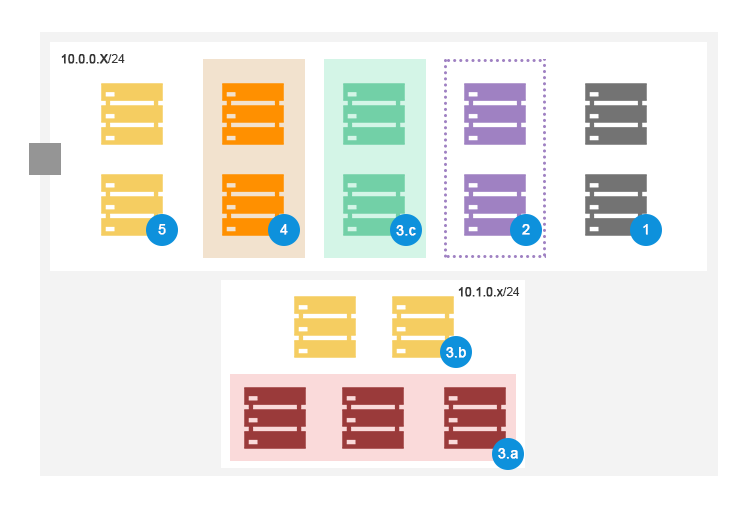
\includegraphics[width=1\textwidth]{images/infrastructure/strategy}}
\label{fig:infrastructure-strategy}
\caption{Estratégia de concepção da infraestrutura}
\end{figure}

Como se pode verificar, a infraestrutura é contituída por várias componenentes, responsáveis pela execução e gestão de vários serviços, estes que serão enunciados mais à frente. Antes de se tornar clara cada componente, tenha-se a noção dos seguintes pressupostos:

\begin{itemize}
	\item A numeração está de acordo com o fluxo de arranque do serviço;
	\item As áreas a branco são representações das sub-redes da infraestrutura, acompanhadas pelo \emph{IP} nos cantos superiores;
	\item As áreas coloridas são representações das componentes onde a escalabilidade horizontal pode ser realizada e, por isso, onde se torna mais importante efetuar essa acção;
	\item O tracejado que engloba servidores corresponde a um \emph{cluster} de máquinas;
	\item Cada cor corresponde a uma componente. Note que um tipo de componente pode ser encontrada em vários pontos da infraestrutura, como acontece com a cor amarela.
\end{itemize}

Tendo em conta estes pressuposts e de acordo com a figura anterior, a infraestrutura encontra-se organizada da seguinte forma:

\begin{enumerate}
	\item \emph{Storage} que promove a persistência de dados de uma forma segura, com replicação e alta disponibilidade.
	\item \emph{Service Cluster} é um \emph{cluster} de alta disponibilidade responsável por tornar disponíveis e acessíveis os serviços que usufruem da componente anterior, abstraindo a posição destes nas máquinas que o compõem.
	\item \emph{Application} é o conjunto de servidores que executa e suporta toda a aplicação.
	\begin{enumerate}
		\item \emph{Application Cache Servers} mantêm alguns dados relevantes para a aplicação em memória, o que permite um acesso mais rápido do que à \emph{Storage}
		\item \emph{Load Balancers} são responsáveis pela distribuição de carga pelos \emph{Application Cache Servers}
		\item \emph{Application Servers} executam a aplicação e servem as suas funcionalidades;
	\end{enumerate}
	\item \emph{Web Servers} são responsáveis por interpretar os pedidos \emph{HTTP} e reencaminhá-los para a aplicação nos \emph{Application Servers}
	\item \emph{Load Balancers} filtram, distribuem a carga dos pedidos \emph{HTTP} pelos \emph{Web Servers} e reencaminha-os para a aplicação nos \emph{Application Servers}
	\item \emph{Virtual IP} fixo, que pode ser utilizado para anexar a um domínio, como \emph{www.billmate.com}. É uma abstração do acesso ao serviço, através do exterior.
\end{enumerate}

De seguida, explicar-se-ão, de uma forma mais detalhada estes componentes e os serviços que os compõem.
